\chapter{Introduction}{}
\label{sec:intro}

% \lettrine[lraise=0.1, nindent=0em, slope=-.5em]{T}{HE RECENT RISE} of Internet-scale code search engines---e.g., Seahawk~\cite{Bacchelli:2012dl}, Portfolio~\cite{McMillan:2011wq}, Sourcerer~\cite{Bajracharya:2006vn}, Koders~\footnote{\url{http://www.koders.com}}---has catapulted search-driven development from backwater to ubiquity, and given rise to an active research community focused on this phenomena~\cite{Bajracharya:2009fj, Bajracharya:2010iy, Bajracharya:2011kw}. The increased prevalence of such engines has given search-driven development more diverse sources of information---e.g., from open sourced code to code snippets from StackOverflow~\footnote{\url{http://www.stackoverflow.com}}---and a more open platform---the Internet~\cite{GallardoValencia:2009gr, GallardoValencia:2010ij, Ying:2012tr}. This new condition has enabled developers to build applications opportunistically by iteratively finding, combining, and reusing online source code~\cite{Brandt:2008wi, Brandt:2009jb, Ying:2012tr}. This opportunistic way of building applications is not easy because searched sources are large, in most cases unsuitable, and quite often unrelated~\cite{GallardoValencia:2009gr}. Consequently, if search-driven development were to be established as best practice, then the time involved in deciding the best search result(s) to reuse must be minimized.

\lettrine[lraise=0.1, nindent=0em, slope=-.5em]{T}{HE RECENT RISE} of Internet-scale code search engines---e.g., Seahawk~\cite{Bacchelli:2012dl}, Portfolio~\cite{McMillan:2011wq}, Sourcerer~\cite{Bajracharya:2006vn}, Ohloh code~\footnote{\url{http://code.ohloh.com}}---has catapulted search-driven development from backwater to ubiquity, and given rise to an active research community focused on this phenomena~\cite{Bajracharya:2009fj, Bajracharya:2010iy, Bajracharya:2011kw}. The increased prevalence of such engines has given search-driven development more diverse sources of information---e.g., from open sourced code to code snippets from StackOverflow~\footnote{\url{http://www.stackoverflow.com}}---and a more open platform---the Internet. This new condition has enabled developers to build applications opportunistically by iteratively finding, combining, and reusing online source code~\cite{Brandt:2008wi, Ncube:2008fm, Brandt:2009jb, McMillan:2012dj}. This opportunistic way of building applications is not easy because searched sources are large, in most cases unsuitable, and quite often unrelated~\cite{GallardoValencia:2009gr}. Consequently, if search-driven development were to be established as best practice, then the time involved in deciding a best search result to reuse must be minimized.

Obviously, code search all by itself won't solve the whole problem. In fact, code-only searching misses out on certain human abilities that are important in search-driven development, such as the ability to quickly identify---based on knowledge and experience---a better result among many, and to change the found code to better reflect what existed only in the human mind. Previously published work has started tackling these issues from different directions\footnote{Two of these directions are the most popular: enhancing search technology~\cite{Bajracharya:2010um, Gysin:2010kt, McMillan:2011cm, McMillan:2012dj, Ying:2012tr}, and coupling Web search and crowdsourced input with IDEs~\cite{Bacchelli:2012dl, Brandt:2010tp, Hartmann:2010hx, Hoffmann:2007wo, Oney:2012ge, Wightman:2012gc}}; each with unique strengths and weaknesses. What all these directions have in common is that developers have to try the code example first, before they know its suitability. In fact, developers are given no guidance as to which result may be a best fit for their code in progress, beyond the existing ranking values. This limitation is one of the reasons why search-driven development is so cumbersome, and ultimately can be a drain on one of the most precious resources in software development: time. 

% Previously published work has tried to tackle the above problem from different directions. Two of these directions are the most popular. One direction focuses entirely on enhancing search technology~\cite{Bajracharya:2010um, Gysin:2010kt, Mandelin:2005uj, McMillan:2011cm, McMillan:2012dj}, while the other direction focuses on coupling Web search and crowdsourced input with IDEs~\cite{Bacchelli:2012dl, Brandt:2010tp, Hartmann:2010hx, Hoffmann:2007wo, Wightman:2012gc}. Although these directions focus on addressing the trustability and relevance of search results, none of them adequately address the \emph{suitability} of these results. In other words, developers are given no guidance as to which result may be a best fit for their code in progress, beyond the existing ranking values. Precisely, developers still have to \emph{manually} mine and try all these ranked results before they could possibly realize their usefulness---or uselessness. This limitation is one of the reasons why search-driven development is so cumbersome, and ultimately can be a drain on one of the most precious resources in software development: time.

An increasingly familiar example of search-driven development arises when modifying a program to support a particular set of functionality. Sometimes, the task is to reuse external third-party libraries, or to support algorithms with specific performance characteristics. Other times, a developer may want to support a feature implemented by code with a conflicting API. A good example would be adapting a sentiment analysis tool (that uses the Twitter API) to use the Facebook API. This type of tool permits the classification of opinions in text (e.g., status updates in Twitter) into categories like ``positive'' or ``negative.'' 

The rise of open source software and code search tools makes it simpler to find large sets of relevant examples. Easily, one could find around fifty platform-specific Facebook libraries and a few dozen general-purpose Facebook libraries on Github\footnote{\url{http://www.github.com}}, each with differences and similarities. However, tool support for determining if any source code found in those libraries is a best fit for one's code is either inchoate or non-existent. This makes the task of locating any suitable code overwhelming, tedious, and error prone. %The consequent effect of this problem is a significant reduction of productivity.

So the real problem with the above scenarios is their uncertainty. Developers cannot plan the impact of choosing a code example on their current work until they have tried it. But then it’s too late. The disturbance in the developers' workflow has already occurred and resulted in time wasted.

%%Both Facebook and Twitter are popular services with different purpose and functionality, and yet they share a common feature: text-based status updates. This suggests that there is an exploitable correspondence between the ``status updates'' source code of the two services' APIs. Due to these services' popularity in the open source world\footnote{Search for Twitter or Facebook at \url{www.github.com}.}, it is common for one to rely on the proliferation of open source software and the availability of code search tools to find large sets of relevant examples~\cite{Reiss2009}. These are examples that could potentially help changed the sentiment analysis tool to use the Facebook API. Even if one were to overlook these dependencies, the absence of tool support for \emph{anticipating} the usefulness of retrieved examples makes retargeting\footnote{Retargeting is the process of altering source code to fit an alternate context.} tasks heavyweight, tedious, and error-prone. %All these factors combined imply that code search all by itself doesn't solve the whole problem.%%In the context of modifying the bullying detection program, the absence of such tool support could lead to the developer going beyond the time allocated for the task or not finishing the task at all. This is augmented, in part, by the %%developer constantly switching \emph{back and forth} between results evaluation and further searches. 
% 
% Obviously, code search all by itself doesn't solve the whole problem. In fact, code-only searching misses out on certain human abilities that are important in search-driven development, such as the ability to quickly identify better results among a myriad of retrieved examples, to demarcate feasible regions of code, and to transform results into code that resembles what existed only in the human mind. Do note there are systems, such as~\cite{Bajracharya:2010um, Gysin:2010kt, Hartmann:2010hx, McMillan:2012dj, Sawadsky:2011eh, Wightman:2012gc} that are starting to address these issues; each with unique strengths and weaknesses. However, tool support for predetermining the usefulness of any search result based on the above abilities is inchoate, leaving developers to perform the retargeting\footnote{Retargeting is the process of altering a source code to fit an alternate context} the old fashioned way. The consequent effect of these limitations is a surprisingly significant reduction of productivity~\cite{Cypher:2010ub, Gysin:2010kt}.

To alleviate the problem imposed by the above limitation, I propose a new approach in search-oriented architecture, called \emph{Snippet Retargeting Approach} or simply \uppercase{SnipR}. \uppercase{SnipR} complements code search with code retargeting capabilities. These capabilities are semi-automatic program transformations that convert the structure of one snippet into the structure of another. They are learned from code examples (i.e., searched results) and encapsulated in a representation that could be accessed algorithmically---i.e., a code mapping (see Chapter~\ref{chap:algorithms} for details). Their intent is to help expedite the process of determining if a source code is a best fit---i.e., suitable---by giving developers the means to ``wipe the dirt off a code example so they can see beyond''\footnote{The original quote is ``wiping the dirt off a window so you can see beyond.'' It first appeared on Martin Fowler's Refactoring book~\cite{Fowler:1999vp} to describe the early code changes made to a program to improve the developers' understanding of the program.}. It doesn’t take long for the application of these capabilities---in conjunction with other searching actions---to become a virtuous loop (Figure~\ref{fig:retargeting}) where developers check their retargeting ideas as they think of them, change the found code to better reflect their understanding, and select only the snippets they can justify as suitable. That is, the found code is retargetable and the cognitive distance~\cite{Krueger:1992wf} to understand how to use it is minimal. Consequently, it is hypothesized that when developers include retargeting in their code search practice, they can confidently justify the suitability of a found code example.     

\uppercase{SnipR}' code retargeting capabilities are embedded within the \emph{query processing} step of a code search engine in order to modify retrieved source code. Each query, issued by a developer, is interpreted in two ways. First, as a request for a particular result set. Second, as a request to retarget relevant bodies of code in that set---e.g., to modify a retrieved code example to use an alternative API. In this context, the suitability of a code example can now be determined by applying these program transformations---code retargeting---to it and to later and similar examples. 

This type of code retargeting is performed in place, without requiring developers to leave the search interface. With regard to the sentiment analysis tool example, \uppercase{SnipR} allows an iterative approach for changing the tool's code from using the Twitter API to using the Facebook API. One would issue a query; inspect the result set; demarcate code blocks to be transitioned; retarget examples; inspect the modified examples; and reject unsuitable examples. At this point, one would rely on the suitability of these candidates to identify the next course of action.

\begin{figure}[!ht]
    \centering
    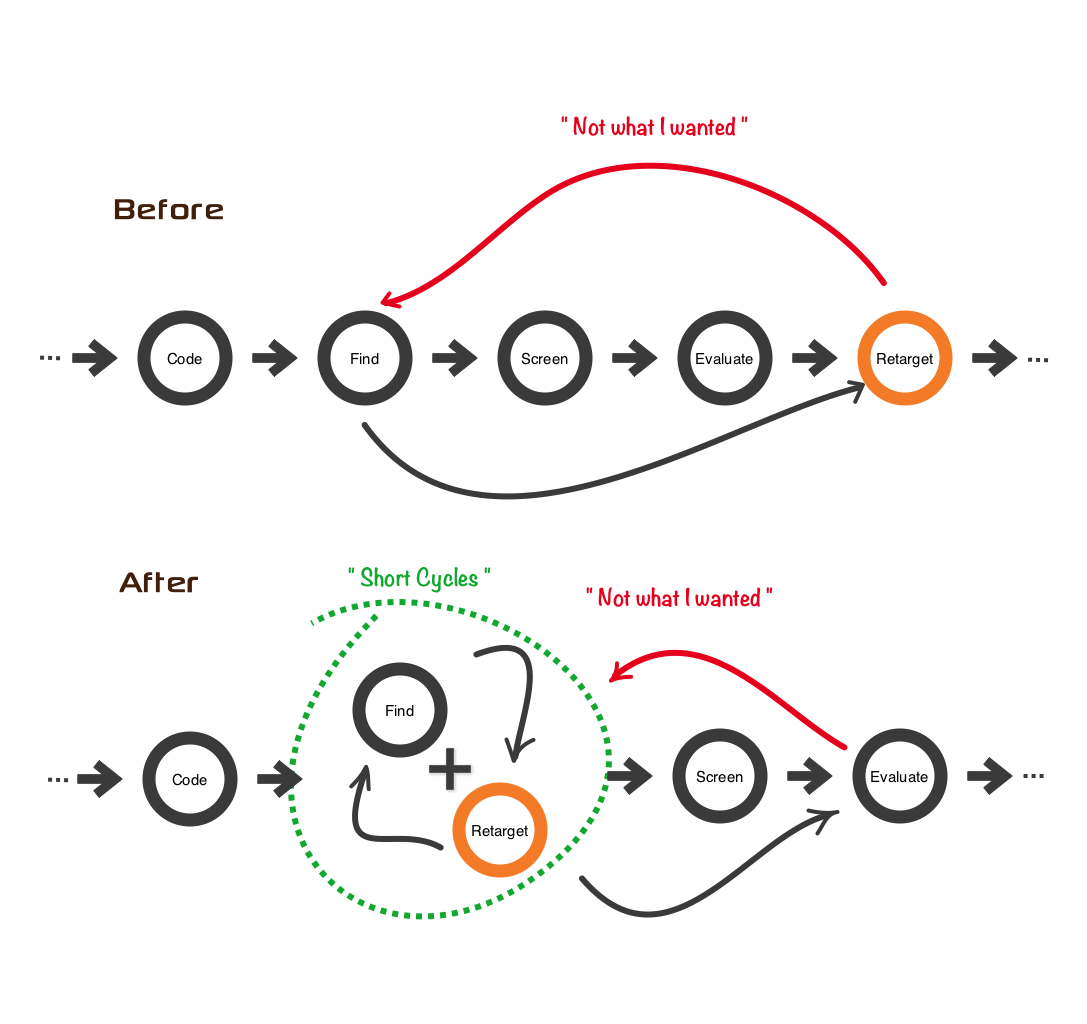
\includegraphics[width=\textwidth]{images/searchprocess}
    \caption{Search Process before and with \uppercase{SnipR}.}
    \label{fig:retargeting}
\end{figure}
% \pagebreak

Figure~\ref{fig:retargeting} illustrates the search process before and with \uppercase{SnipR}. A pre--\uppercase{SnipR} scenario requires effort from developers to find and select the most promising examples (i.e., screening), and to study each one of them before eventually consuming them in the IDE (e.g., start with code modification actions). If the resulting code is not the desired code, then the search process is restarted by the developer. In the \uppercase{SnipR} scenario, developers engage in a virtuous loop where they find and select only suitable choices; i.e., examples that can be retargeted. This minimizes the number of iterations in the search process, since the developer is only dealing with suitable choices---choices that would be easier to consume in the IDE.

In retrospect, if the time required to determine the most suitable results is minimized by code retargeting, then the effort of integrating these search results is also minimized. If retargeting is unsuccessful, then the developer will continue searching for more examples and retarget as needed. Overall, \uppercase{SnipR} will allow code queries and retargeting requests\footnote{The everyday search box would be enhanced with command line power; e.g., code manipulation commands.} to be intermixed---or used separately---by developers to explore potential code changes on the retrieved results (See \uppercase{SnipR} scenario in Figure~\ref{fig:retargeting}). This offers two important advantages. If the developer is retargeting the source as they search, then the evaluation results of retargeted examples are available immediately, which saves valuable human time searching for an appropriate example code. If the developer is choosing what example code to retarget, then the evaluation results can inform the decision, pointing the developer to the best choice. This is an attractive proposition and very different to the directions taken by previous work. It is attractive because one can figure out as early as possible if a code example is appropriate or not. It is different because one can do this without requiring to leave the search interface.
% This proposed approach suggests an environment where human and search engine help each other out and accept the challenge of retargeting code on the spot.  

This work proposes the following solutions to the aforementioned problem:

\begin{itemize}
\item Twist, a language for interacting with search results, and applying retargeting operations to source code.
\item An algorithm for learning code mappings from code examples. 
\item A set of retargeting operators well suited for manipulating example code; i.e., applying code mappings and displaying error messages if the mappings cannot be applied.
\item A realization of the \uppercase{SnipR} conceptual architecture in a working system for code search and retargeting. 
\item An evaluation of the efficiency of the \uppercase{SnipR} approach versus existing approaches for doing code search and retargeting tasks. 
\end{itemize}

These solutions are the expected contributions of this work in search-driven development and thus in software engineering. 

\fancybreak{\pfbreakdisplay}

\section{Research Questions}
\label{sec:questions}

An essential part of knowing what kind of search-driven tools could help developers find the right examples to reuse is knowing precisely why search-driven development is so difficult. I would examine this question by answering the following guiding questions: 

\begin{itemize}
	
	\item[RQ1] What kind of \uppercase{SnipR} commands could be invoked directly from the search 
	box? 
	
	The aim is to design a set of retargeting commands that could be invoked by developers from the 
	search box, without losing any sight of their current search goal. This design should balance 
	two inter-related principles: simplicity and flexibility. For simplicity, SNIPR will provide 
	most of the mechanisms for expression and control of changes that could be made to modules 
	(methods that implement an API). This involves discovering the fundamental concepts of 
	retargeting modules, to extract them from their various reincarnations, and to present them in a 
	pure and distilled form. This form will be inspired by the syntax of the Io programming 
	language. For flexibility, a simple language for combining, and executing code retargeting 
	commands will be developed. This language's goal is to extend \uppercase{SnipR}'s availability 
	functionality. To evaluate simplicity, a user study and a survey will be performed. For 
	flexibility, the statistics on the use and execution effort for supporting and using different 
	commands will be reported.
		
	% That is, it should resemble the language used by developers when 
	% 	modifying source code, and allow a reasonable set of code changes to be expressed. By applying a 
	% 	simple but well principled rule, I would be able to decide when I have completed this question: This question is 
	% 	complete when I have stopped finding reasons to change any of the already defined commands.
	% 	
	% \item[RQ1] How does \emph{SnipR} compare to existing search-driven development 
	% 	systems~\cite{Bajracharya:2010um, Gysin:2010kt, Hartmann:2010hx, McMillan:2012dj, Sawadsky:2011eh, Wightman:2012gc} and are there any decisive factors in deciding on the approach or 
	% 	system to be used for search-driven development? 
	% 	
	% 		
	% 	I will show \emph{SnipR} is less a competitor to any of the above referenced systems and more 
	% 	of a platform. It is an effective way to improve the search for suitable 
	% 	examples, but any number of other development tools can come into play after 
	% 	the retargeting of the first few examples.  
	% 	%\emph{SnipR} will target a situation where the users don't know what they want until 
	% 	%they see it. There's no prior knowledge about the usefulness or uselessness of those 
	% 	%examples, and there is limited time and resources.
	% 	
	\item[RQ2] How expensive is it to retarget (part of) found source code each time?
	
	This question is about the performance (in terms of computational throughput) of the code 
	retargeting algorithms. In other words, this is about how long it will take the code retargeting 
	algorithms to apply the appropriate code mappings to any found source code. Code retargeting is 
	an operation that can operate on a single result or an entire result set. Therefore, this 
	operation requires that those cases where code mappings can be learned and/or applied are 
	carefully identified. This will prevent any unnecessary work from happening as matched code 
	examples are being returned by the query engine. To evaluate the performance of this algorithms, 
	a set of microbenchmarks will be implemented, and the obtained statistics reported.
	
	% Per Jim's comment on Sunday Oct 28, 2012 
	% \item[RQ2] What is the impact on programming time when retargeting is done at the 
	% integrated development environment versus when it is done at the search interface?  
	% 
	% Significant amount of time is lost when developers must move retrieved code from one 
	% environment to another. The screening and changing of the retrieved code at the 
	% search interface would minimize any back and forth movement between results 
	% evaluation and further searches.
	
	\item[RQ3] Where does \uppercase{SnipR} belong within the query processing step of any 
	modern code search engine?
	
	The answer to this question will be based on a working system for code search, such as 
	Sourcerer\cite{Bajracharya:2006vn} Internet-scale code search engine. This system will 
	be updated with \uppercase{SnipR}. Then, this work will rely on any experimentation performed 
	on the updated system to answer this question. 
	% 
	% \item[RQ3] Will productivity time increase when using SnipR versus not using SnipR?
	% 
	% Retargeting time is directly linked to integration time. If integration time goes 
	% down, then productivity time goes up. Since SnipR is trying to minimize 
	% integration time, then productivity is likely to increase.
	
	% \item[RQ4] How does the performance---in terms of the time to perform a more complete 
	% code search task---of a system using SnipR compare to systems where SnipR is not 
	% available?
	% 
	% \item[RQ4] How does the performance---in terms of the time needed to perform a more complete 
	% code search task---of the SnipR approach compare to the current approaches of code search? 
	
	\item[RQ4] How does the time needed to perform a more complete code search task of the 
	\uppercase{SnipR} approach compare to the current approaches of code search? 
	
	If the developer is retargeting the source in advance, then the evaluation results of 
	retargeted examples are available immediately (See \uppercase{SnipR} scenario in 
	Figure~\ref{fig:retargeting}). This immediate feedback saves valuable time searching for an 
	appropriate example code. As a result, by getting immediate feedback, the developer gets the 
	work done more quickly. This will hold true only if \uppercase{SnipR}'s retargeting operations 
	are efficient, which will be demonstrated by answering RQ2.
	
	% 
	%  
	% \item[RQ4] Will there be a productivity boost when using \emph{SnipR} versus not using \emph{SnipR}?
	% 
	% Retargeting in advance is directly linked to minimizing integration time. If integration time goes 
	% down, then productivity---the time required to write a fixed amount of code---goes up. Since the 
	% retarget code produced by \emph{SnipR} is the best fit, then the integration of such code is faster than the 
	% integration of less suitable code; i.e., code that relies only on ranking values. Consequently, I anticipate a 
	% boost in productivity.
		
	% \item[RQ4] Would the very way code manipulation is piggy-backed to query processing 
	% and advised by users' queries lead to a successful code integration?
	% 
	% If the most suitable results are found by retargeting, then the odds of code 
	% integration success are increased. By validating the SnipR approach 
	% and results in practice, I would be able to confirm whether the retargeted code 
	% produced by SnipR was successfully integrated.
\end{itemize}

All the work proposed in this document is motivated by a grander vision of where the next generation of programming practices and behaviors involving code search could take us. The time is ripe to change the role of code search as a development tool from a mere supporting role to a starring role.
\fancybreak{\pfbreakdisplay}

\section{Outline}
\label{sec:outline}

The rest of this document is structured as follows. In Chapter 2, I discuss related work.
Once the related is covered, I present the foundations of the Snippet Retargeting Approach in Chapter 3, 4, and 5. Chapter 3 describes the policy behind \uppercase{SnipR}. In Chapter 4, I describe the learning algorithm for building code mappings from code examples. This chapter also describes two procedures needed to set up \uppercase{SnipR}. In Chapter 5, I present Twist, a language for interacting with search results, and combining
and executing code retargeting operations. In Chapter 6, the proposed solutions, including the evaluation, and the work timeline are presented. Finally, Chapter 7 concludes the proposal.